\chapter{Graver bases} \label{literature}

\lhead{\emph{Graver bases}}  % Set the left side page header


Before introducing the concept of Graver basis of a matrix, we define a partial order $\sqsubseteq$ in $\mathbb{R}^n$ by $u \sqsubseteq v$ if $u_i \cdot v_i \geq 0$ and $|u_i| \leq |v_i|$ for all i. Note that the condition $u_i \cdot v_i \geq 0$ means that $\sqsubseteq$ can only compare \textit{sign compatible} vectors, i.e., with the same sign componentwise. The Graver basis of a matrix is the set of minimal elements (for this order $\sqsubseteq$) in its integral kernel excluding zero. Formally: 

\begin{definition}[\textbf{Graver basis}]
The Graver basis ($\mathcal{G}(A)$) of a given matrix $A \in \mathbb{Z}^{mxn}$ is defined as the set of $\sqsubseteq$-minimal elements in $\{z \in \mathbb{Z}^n: Az = 0, z\neq0\}$.%$ker(A) \setminus \{0\}$.\\
\end{definition}

\vspace{-5pt}
Graver bases were initially defined as \textit{universal integral test set} in \cite{GRAVER:1975} by Jack. E. Graver, in 1975. They often appear also defined in an equivalent way as the nonzero indecomposable elements in $ker(A)$. Indecomposable in the sense that they can not be expressed as the sum of two sign compatible vectors. It's easy to see the equivalence of both definitions.

Now that Graver bases are formally defined, we present their main properties in the form of propositions which will be the theoretical basis for the algorithms presented in the next sections.

\begin{proposition}
For every matrix A, $\mathcal{G}(A)$ is a finite set.
\end{proposition}
\vspace{-20pt}
\begin{proof}
Dickson's lemma states that every subset of $\mathbb{N}^n$ has a finite number of minimal elements (with the order $\leq$ componentwise). It's easy to see that this implies that the integral kernel of A (excluding zero) has a finite number of $\sqsubseteq$-minimal elements in every orthant. As the elements in different orthants are not comparable we have that $\mathcal{G}(A)$ is the union of $2^n$ finite sets, concluding the proof.
\end{proof}

Unfortunately, the cardinality of $\mathcal{G}(A)$ may be exponential in $n$, the number of columns of $A$. This of course limits the explicit computation and usage of the Graver basis to only certain cases but of course doesn't limit its theoretical properties. The most important of these properties is expressed in the following proposition:

\begin{proposition}
Every integral element in $ker(A)$ can be expressed as positive integral linear combination of sign compatible elements in $\mathcal{G}(A)$.
\end{proposition}
\vspace{-20pt}
% TODO: Review!
% TODO: Compare with proof of lemma 4.2 [Onn-Convex_IP-2007]!
\begin{proof}
The proof is by induction in the $\ell_1$ norm. For the base case we see that given $u \in \mathbb{Z}^n\cap ker(A)$ such that $||u||_1 = 1$ then $u$ belongs to $\mathcal{G}(A)$ and the result holds.

For the induction case lets suppose the result is given up to k and take $u \in \mathbb{Z}^n\cap ker(A)$ such that $||u||_1 = k$. Again, if $u$ is minimal in $\mathbb{Z}^n\cap ker(A) \setminus \{0\}$ the result is clear so let's suppose this is not the case. Therefore it exists $u_1$ s.t. $u_1 \sqsubseteq u, u_1 \neq u$. We take $u_2 = u - u_1$. Note that thanks to the definition of $\sqsubseteq$ $u$, $u_1$ and $u_2$ are sign compatible and thanks to $u \neq u_1$ necessarily  $||u_1||_1,||u_2||_1 \leq k$. With this appreciations, the proof concludes after applying the induction hypothesis:\\
\vspace{-30pt}
\begin{center}
    $u = u_1 + u_2 = \sum \alpha_{1i}g_{1i} + \sum \alpha_{2i}g_{2i} = \sum \alpha_{j}g_{j}$
\end{center}
\end{proof}

This proposition is the reason why Graver bases were introduced as \textit{universal integral test set}. It ensures that, given any feasible point, the whole feasible region can be expressed in terms of elements in $\mathcal{G}(A)$. Note that thanks to requiring positive coefficients and sign compatible elements we avoid cancellations in every component. 

In the next proposition we see how, thanks to this property, we can do an optimality test for any feasible point using only elements in the Graver basis.

\begin{proposition}
Given a feasible point $z$ of the IP, $z$ is not optimum if and only if there exists $g \in \mathcal{G}(A)$ s.t. $c^tg > 0$ and $l \leq z + g \leq u$.
\end{proposition}
\vspace{-20pt}
\begin{proof}
If there exists $g \in \mathcal{G}(A)$ (therefore $\in ker(A)$) $s.t. c^tg > 0$ is clear that $z + g$ is a feasible point which strictly improves the objective function, so $z$ is not an optimum. 

For the other implication, if z is not an optimum we can take a feasible point $y$ improving $z$, then $y - z$ verifies the hypothesis of the previous proposition so there exist $g_i \in G(A)$, $\alpha_i \geq 0$ s. t. $0 < c^t(y - z) = \sum \alpha_i c^t g_i$ and it's then clear that exists at least one $g_i \in \mathcal{G}(A)$ verifying $c^tg_i > 0$. Finally, thanks of $\alpha_i \geq 0$ and $g_i$ being sign compatible with $y - z$ we have that for all $i$, $l \leq z \leq z + g_i \leq z + \sum \alpha_i g_i = y \leq u$.
\end{proof}

\section{Graver Basis greedy augmentation algorithm}

We now consider how to solve the general IP with the help of Graver bases. Note that proposition 2.4 doesn't only give us an optimality test but also provide us an improvement direction if the feasible point is not optimal. We can follow that improvement direction to get a better feasible point and then repeat this process. That is the idea of the following procedure (idea introduced in \cite{GRAVER:1975}):

\textbf{General IP algorithm using Graver basis}
\vspace{-8pt}
\begin{enumerate}
    \item From a feasible solution $z_i$
    \item Find $g^*$ optimum for the sub-problem: \vspace{4pt}\\
          $max\{c^tg : g \in \mathcal{G}(A), l \leq z_i + g \leq u \}$ \vspace{4pt}
    \begin{itemize}
        \item $c^tg^* \leq 0 \implies z_i$ optimal solution.
        \item $c^tg^* > 0 \implies$ $g^*$ improvement direction, loop back to 1 with:\\ $z_{i+1} = z_i + \lambda \cdot g^*$ with the biggest $\lambda$ respecting the bounds.
    \end{itemize}
\end{enumerate}
%\hspace{15pt} [References??]

We can affirm that it's an algorithm, i.e., it finishes in a finite number of steps, thanks to the lower and upper bounds $l$ and $u$. We can assume they are finite and, this way, the objective function is also bounded. Since every iteration we are strictly increasing the objective function, no infinite loop is possible. As is well known, it is always possible to add suitable polynomial upper and lower bounds without excluding some optimal solution if any, so assuming $l$ and $u$ to be finite is no loss of generality.

% TODO: href style!
% TODO: Maybe proposition with the complexity ??
% TODO: Improve \cite{...} (Theorem x.y) ??
The question that arises now is the complexity of this algorithm. It was analyzed in \cite{LHOW:2006} (Theorem 3.3) showing that it's polynomial. This of course doesn't mean we have a polynomial algorithm for the general IP, it means that, given an IP along with its Graver basis, we have a polynomial algorithm in this input size. The complexity of the problem remains in computing the Graver basis which, as we announced, may be exponential. This makes the algorithm non-viable but for small matrices. In the Appendix A we go further to analyze how to compute the Graver basis of a given matrix and we introduce the tool \href{https://4ti2.github.io/}{4ti2}.

% TODO: Textbf for the complexity (last sentence) ??
Another way to estimate the complexity of the algorithm is using \cite{HOW:2009} (Theorem 2.b), which states that the number of augmentation steps is polynomial. Since once obtained the Graver basis the cost of each augmentation step is in the order $n \cdot |\mathcal{G}(A)|$ (search over $\mathcal{G}(A)$), it's clear that the algorithm is polynomial in $n \cdot |\mathcal{G}(A)|$.



\section{Graver Basis norm bounds}

Up to this point we have seen how Graver bases allow a straightforward algorithm for the general IP. However, we have seen that its main drawback is that it requires the explicit computation of the Graver basis. In this section we show how we can avoid computing it thanks to bounds on the $\ell_1$-norm of the Graver basis elements.

\begin{proposition}[\textbf{Graver basis bounds}]
Given $A \in \mathbb{Z}^{mxn}$ and $\Delta$ an upper bound for the absolute value of each component of $A$, for every $g \in \mathcal{G}(A)$:
\vspace{-10pt}
\begin{itemize}
    \item $||g||_1 \leq m^{m/2}\Delta^m\cdot(n - m)$ \hspace{10pt}[Onn 2010]
    \item $||g||_1 \leq (2m \Delta + 1)^m$ \hspace{41pt}[Eisenbrand,Hunkenschröder,Klein 2018]
\end{itemize}
\end{proposition}

We refer to \cite{ONN:2010} and \cite{EISENBRAND:2018} for the proof. Note that both bounds are exponential in the number of rows of $A$ but the second one has the advantage of being independent in the number of columns. 

Why should bounds to the Graver bases help? Because thanks to Proposition 2.4, the search of an improvement direction can be restricted to the elements in the Graver basis and, thanks to the bounds, we can restrict our search space without excluding any element of the Graver basis. This is the idea of the following algorithm (see \cite{HEMMECKE:2011}).

% TODO: Maybe here is the place for the first image!
% TODO: Definitely it would be nice to add the images!

\vspace{10pt}
\begin{figure}[h]
\centering
\begin{minipage}[b]{0.45\textwidth}
    \centering
    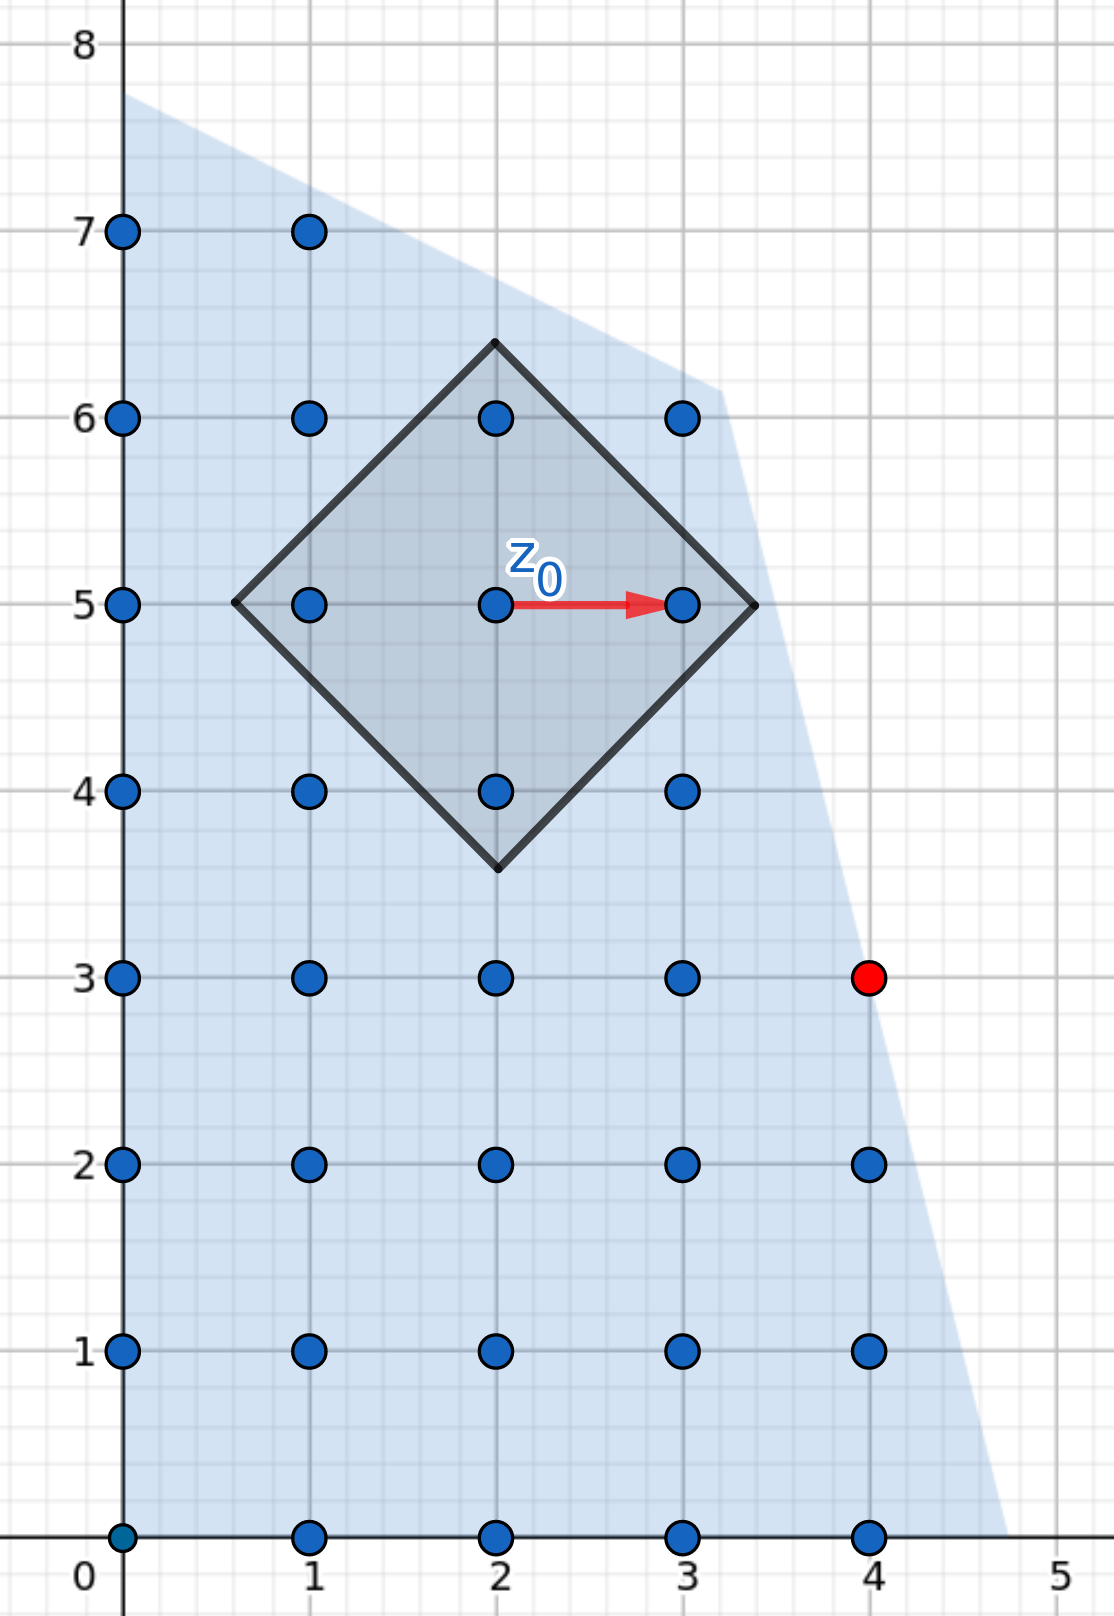
\includegraphics[width=0.9\textwidth]{images/IP(6).png}
    % TODO!
    \caption{Complete this}
\end{minipage}
\hfill
\begin{minipage}[b]{0.45\textwidth}
    \centering
    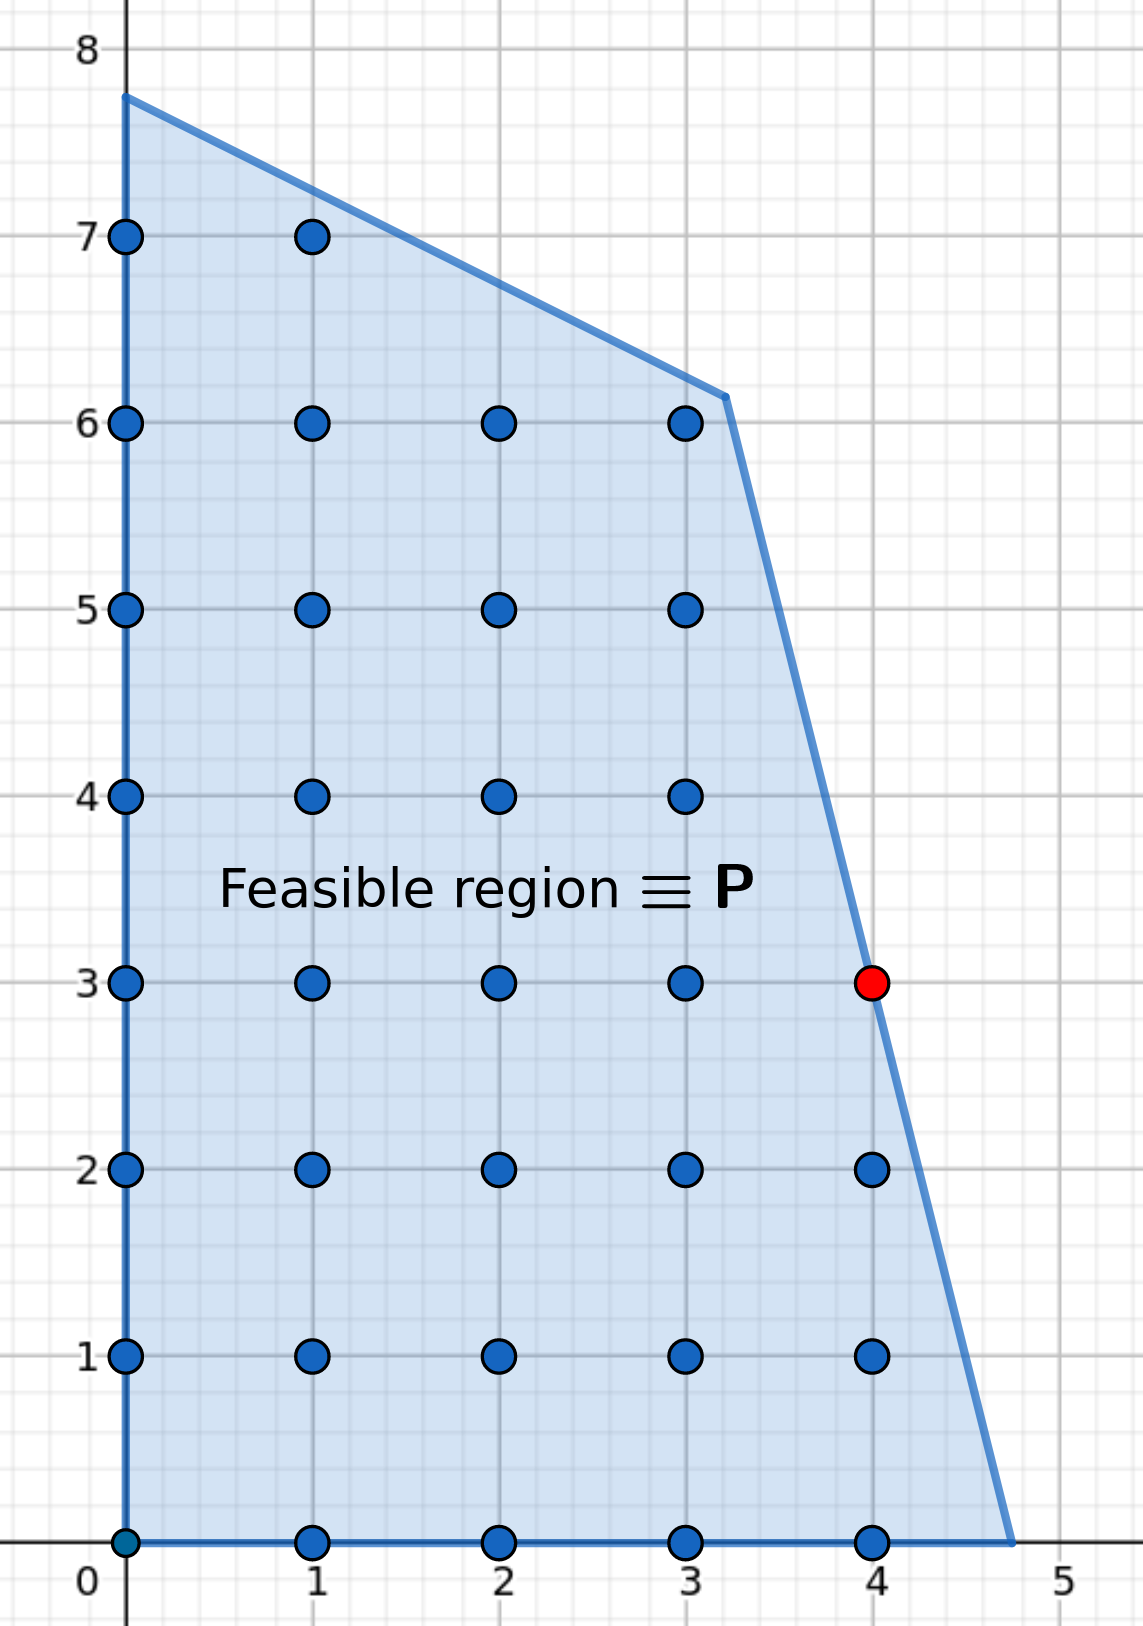
\includegraphics[width=0.9\textwidth]{images/IP(12).png}
    % TODO!
    \caption{Also this}
\end{minipage}
\end{figure}

% TODO: I don't like newpage commands! avoid if possible
\newpage
\textbf{General IP algorithm using Graver basis norm bound}
\vspace{-8pt}
\begin{enumerate}
    \item From a feasible solution $z_i$
    \item Find $g^*$ optimum for the sub-problem: \vspace{4pt}\\
          $max\{c^tg : Ag = 0, l-z_i \leq g \leq u-z_i, g \in \mathbb{Z}^n, ||g||_1 \leq ||\mathcal{G}(A)|| \}$ \vspace{4pt}
    \begin{itemize}
        \item $g^* = 0 \implies z_i$ optimal solution.
        \item $g^* \neq 0 \implies$ $g^*$ improvement direction, loop back to 1 with:\\
        $z_{i+1} = z_i + \lambda \cdot g^*$ with the biggest $\lambda$ respecting the bounds.
    \end{itemize}
\end{enumerate}
%\hspace{15pt} [Hemmecke, Onn, Romanchuk 2013]


As we advanced, the main advantage of this algorithm is that it doesn't require the explicit computation of the Graver Basis. However, the complexity is totally dependent on the added restriction $||g||_1 \leq ||\mathcal{G}(A)||$, and the only bounds we have for the general case are exponential. In this case, the additional restriction to the problem doesn't improves the lower and upper bounds and the complexity is exponential. 

In certain cases we can get a much tighter bound for the Graver Basis elements and this can help us to get a faster algorithm. The N-Fold IP is an iconic example. 